

\chapter{Changing Bases}

This chapter covers the following ideas. The purpose of this chapter is to help you understand different bases can provide useful ways of viewing a linear transformation.


\begin{enumerate}
\item Explain how to describe vectors using different coordinate systems. Be able to change between different coordinate systems, and use these ideas to construct matrix representations of linear transformations.
\item Show that the null space (kernel), column space (image), and eigenspaces of a matrix (linear transformation) are vector subspaces. Be able to extend a basis for these spaces to a basis for the domain or codomain.
\item For square matrices, explain why similar matrices $B=P^{-1}AP$ represent the same linear transformation (just using a different basis). Explain why the determinant, eigenvalues, rank, and nullity of a linear transformation are not dependent upon the basis chosen.
\item Explain how to diagonalize a matrix, as well as explain when it is or is not possible. 
\end{enumerate}





\section{Coordinate Systems}


\subsection{Coordinates relative to a basis}
When we write the vector $\vec u=(2,4,7)$, we are giving the coordinates of the vector relative to the standard basis $E=\{(1,0,0),\,(0,1,0),\,(0,0,1)\}=\{\vec e_1,\vec e_2,\vec e_3\}$. We could write $(2,4,7)$ as a linear combination of these basis vectors by writing $(2,4,7)=2\vec e_1+4\vec e_2+7\vec e_3$. The numbers $2,4,7$ are called the \define{coordinates} of $\vec u$ relative to the standard basis vectors, and they form a vector $[\vec u]_E=(2,4,7)_E$ called the coordinate vector of $\vec u$ relative to the basis $E$.  We use the subscript $E$ to emphasize that the vector $(2,4,7)$ is really just the coordinate vector whose components are the coordinates relative to $E$.  

If instead we use the basis vectors $S=\{(1,1,1),\,(0,1,1),\,(0,0,1)\}$, then since $(2,4,7)=2(1,1,1)+2(0,1,1)+3(0,0,1)$, we write $[\vec u]_S=(2,2,3)_S$ as the coordinate vector of $\vec u$ relative to $S$. We will write $[(2,4,7)]_S = (2,2,3)_S$ to say that the coordinates of $(2,4,7)$ relative to $S$ are $(2,2,3)_S$. The subscript $S$ reminds us which basis vectors we are using for the coordinates.

When we work with polynomials in $P_3(x)$ with standard basis $E=\{1,x,x^2,x^3\}$, the coordinates of $2+4x-5x^2+3x^3$ relative to this basis are $[2+4x-5x^2+3x^3]_E = (2,4,-5,3)_E$. 
If the basis is understood from context, then often we will omit the subscript. The coordinates of the matrix $\bm{1&2&3\\4&-2&0}$ relative to the standard basis $$S = \left\{ \bm{1&0&0\\0&0&0} ,\bm{0&1&0\\0&0&0} ,\bm{0&0&1\\0&0&0} ,\bm{0&0&0\\1&0&0} ,\bm{0&0&0\\0&1&0} ,\bm{0&0&0\\0&0&1} \right\}$$ are simply $\left[\bm{1&2&3\\4&-2&0}\right]_S = (1,2,3,4,-2,0)$ (we didn't put a subscript on the last coordinate vector because the basis was clear from context).

How do you find the coordinates of a vector relative to a basis? We've been doing it in every chapter up till now every time we find reduced row echelon form.  The coordinates of a vector relative to pivot columns are found in the non-pivot columns of rref.  The new thing so far in this chapter is the notation $[\vec u]_S$ for the coordinate vector relative to the basis $S$.  Let's remind ourselves of why row reducing gives the coordinate vector.
\begin{example}
To find the coordinates of $(1,0)$ relative to the basis $S=\{(1,2),\,(3,5)\}$, we need to find coefficients $(x,y)$ such that $$x\bm{1\\2}+y\bm{3\\5} = \bm{1\\0}, \quad \text{or in matrix form} \quad \bm{\cl{1\\2}&\cl{3\\5}}\bm{x\\y}=\bm{1\\0}.$$ 
To solve this system we simply reduce the matrix $\bm{\cl{1\\2}&\cl{3\\5}&\cl{1\\0}}$ to $\bm{\cl{1\\0}&\cl{0\\1}&\cl{-5\\2}}$.
This shows us that the coordinates of $(1,0)$ relative to $S$ are simply $[(1,0)]_S = (-5,2)_S$. 
\end{example}

Notice that the matrix form in the last example showed that if $B$ is a matrix with the basis vectors as columns, then $B[\vec x]_S=\vec x$.
\marginpar{$B[\vec x]_s = \vec x$}

\begin{example} Consider the basis $S=\{(1,2),\,(3,5)\}$. 
\begin{enumerate}
	\item Find the coordinates of $(1,0)$, $(0,1)$, $(3,6)$, $(10,-7)$, and $(a,b)$ relative to this basis.
	\item What vector has coordinates $(3,-2)_S$?
	\item How does the inverse of $B = \begin{bmatrix}1 & 3 \\ 2 & 5\end{bmatrix}$ help find the coordinates of $(a,b)$?
\end{enumerate}
 To answer the first question, we could do five different row reductions.  However, we can do them all simultaneously by inserting the basis vectors as the first two columns of a matrix, augmenting by all of the other vectors, and then reducing: 
$$\begin{bmatrix}
 1 & 3 & 1 & 0 & 3 & 10 & a \\
 2 & 5 & 0 & 1 & 6 & -7 & b
\end{bmatrix}
\xrightarrow{\rref}
\begin{bmatrix}
 1 & 0 & -5 & 3 & 3 & -71 & -5 a+3b \\
 0 & 1 & 2 & -1 & 0 & 27 & 2 a-b
\end{bmatrix}.$$
The coordinates of each vector relative to $S$ are $[(1,0)]_S = (-5,2)_S$, $[(0,1)]_S=(3,-1)_S$, $[(3,6)]_S=(3,0)_S$, $[(10,-7)]_S=(-71,27)_S$, and $[(a,b)]_S=(-5a+3b,2a-b)_S$. 
The columns of the rref give us the coordinates of each vector relative to our basis.

The coordinates $(3,-2)_S$ represent the vector $3(1,2)-2(3,5)=(-3,-4)$. We can write this fact as $[(-3,-4)]_S = (3,-2)_S$.

Notice that in our answer for the first question, we already augmented by $(1,0)$ and $(0,1)$ prior to reducing.  This means that columns 3 and 4 of the rref contain the inverse $B\inv  = \bm{-5 & 3\\ 2 & -1}$.  Also notice that $$B\inv \bm{a\\b} = \bm{-5 & 3\\ 2 & -1}\bm{a\\b} = \bm{-5a+3b\\2a-b}$$ which is precisely the coordinates of $(a,b)$ relative to $S$.  
\end{example}
Notice in the last answer in this example, we see that $B\inv \vec x$ gives the coordinates of $\vec x$ relative to $S$, i.e., $[\vec x]_S = B\inv \vec x$.
\marginpar{$[\vec x]_s = B\inv \vec x$}

The two methods above (using row reduction or inverses) will always give you the coordinates of $\vec u$ relative to the basis $S=\{\vec u_1,\vec u_2,\ldots,\vec u_n\}$ (where $S$ is a basis for ${\mathbb{R}}^n$). 
We will focus on using inverse matrices for the remainder of this chapter, as we need inverse matrices in what follows.  
Much of the work in this chapter involves using inverse matrices to discover new ideas. 

%In summary, if we want to write the vector $\vec v$ as a linear combination of the vectors in $S$, then we need to write $$c_1\vec u_1+c_2\vec u_2+\cdots+c_n\vec u_n = \vec v.$$ In matrix form we write $$\begin{bmatrix}\vec u_1 & \vec u_2&\cdots&\vec u_n\end{bmatrix} \begin{bmatrix}c_1&c_2&\cdots&c_n\end{bmatrix}^T=\vec v\quad \text{or} \quad P[\vec v]_S = \vec v,$$ where $P$ is the matrix whose columns are the basis vectors in $S$. Multiplying both sides on the left by $P^{-1}$ gives us the formula $[\vec v]_S=P^{-1}\vec v$. So we find the coordinates of $\vec v$ relative to $S$ by multiplying the inverse of $P$ on the right by $\vec v$.

\begin{example} 
Given the basis $S=\{(1,2),\,(3,4)\}$, we will find the coordinate of $(3,6)$, $(10,-7)$, and $(a,b)$ relative to this basis by using an inverse matrix.  First, the matrix $B$ and $B\inv$ are
\marginpar{Remember the trick from Section~\ref{sec:quick-2-2-inverse} to easily find the inverse of a 2 by 2 matrix: 

$
\begin{bmatrix}
a&b \\ c&d
\end{bmatrix}^{-1} 
= \frac{1}{ad-bc}
\begin{bmatrix}
d&-b \\ -c&a
\end{bmatrix}
$
}
$$B=
\begin{bmatrix}
 1 & 3 \\
 2 & 4
\end{bmatrix},\quad
B^{-1}=
\ds\frac{1}{-2}\begin{bmatrix}
 4 & -3 \\
 -2 & 1
\end{bmatrix}.$$
  The coordinates relative to $S$ are 
\begin{align*}
[(3,6)]_S&=B^{-1}\bm{3\\6} = \bm{3\\0}_S, \\
[(10,-7)]_S &= B^{-1}\bm{10\\-7}=\bm{-61/2\\27/2}_S,\\
[(a,b)]_S &= B^{-1}\bm{a\\b}=\bm{-2 a+\frac{3 b}{2} \\ a-\frac{b}{2}}_S.
\end{align*}

\end{example}



\subsection{Change of Basis}

If we are given the coordinates $[\vec u]_S$ of a vector $\vec u$ relative to a basis $S$, how do we find the coordinates $[\vec u]_{R}$ of $\vec u$ relative to a different basis $R$? 
We can start by writing everything in terms of a single basis (often the standard basis).
Let $B$ be the matrix whose columns are the basis vectors of $S$ (relative to the standard basis $E$). 
Let $C$ be the matrix whose columns are the basis vectors of $R$ (relative to the standard basis $E$). 
For any vector $\vec u$, whose coordinates relative to the standard basis are $[\vec u]_E$, we write the two equations $$B[\vec u]_S=[\vec u]_E\quad \text {and}\quad C[\vec u]_{R}=[\vec u]_E.$$ 
We equate the left side	of each equation to obtain the matrix equation 
$$B[\vec u]_S=C[\vec u]_{R}.$$ 
Multiplication on the left by $C^{-1}$ gives $$C^{-1}B[\vec u]_S=P[\vec u]_S=[\vec u]_{R}.$$  
You can think of this transformation $P$ as a composition of transformations, $P[\vec u]_S=C\inv (B[\vec u]_S)=C\inv [\vec u]_E=[\vec u]_R$, or in words, first convert $[\vec u]_S$ to standard coordinates $[\vec u]_E$, and then convert to coordinates relative to $R$, $[\vec u]_R$.

The matrix $P=C^{-1}B$ is often called the ``change of basis matrix from $S$ to $R$,'' or the ``change of coordinate matrix from $S$ to $R$.''  To transform from the old basis $S$ to the new basis $R$, we just multiply by $P$: $P[\vec u]_S=[\vec u]_{R}$. The change of basis matrix $Q$ from $R$ to $S$ inverts this process, so it is $Q=P^{-1}=B\inv C$.

\begin{example}
Consider the two bases for the plane $\mathbb{R}^2$: $$S=\{(2,1),\,(3,-2)\}\quad \text{and}\quad R=\{(1,0),\,(2,-1)\}.$$ 
\begin{enumerate}
	\item Find the coordinates of $(-1,3)_S$ relative to the basis $R$ by finding the change of basis matrix $P$ from $S$ to $R$, 
	\item Find the coordinates of $(-1,3)_{R}$ relative to the basis $S$ by finding the change of basis matrix $Q$ from $R$ to $S$, and 
	\item Verify that $Q=P^{-1}$.
\end{enumerate}
\begin{enumerate}
	\item Let 
	$B=
\begin{bmatrix}
 2 & 3 \\
 1 & -2
\end{bmatrix}
$
and 
	$C=
\begin{bmatrix}
 1 & 2 \\
 0 & -1
\end{bmatrix}
$ (the matrices whose columns are the basis vectors $S$ and $R$, respectively).  We know that $B \bm{-1\\3}_S = \bm{7\\-7}=\vec u$ is the actual vector we are trying to represent in terms of the basis $R$.  To find the coordinates relative to $R$, we write $B \bm{-1\\3}_S = C[\vec u]_{R}$, or $C^{-1}B \bm{-1\\3}_S= [\vec u]_{R}$, where 
$C^{-1} = 
\begin{bmatrix}
 1 & 2 \\
 0 & -1
\end{bmatrix}
$. 
The change of basis matrix $P$ from $S$ to $R$ is 
$C^{-1}B =  
\begin{bmatrix}
 4 & -1 \\
 -1 & 2
\end{bmatrix}
$ which means that $[\vec u]_{R}= P\bm{-1\\3} = \bm{-7\\7}_{R}$. So the vector with coordinates $(-1,3)_S$ relative to $S$ is $(7,-7)$ which has coordinates $(-7,7)_{R}$ relative to $R$.

\item
We know that $C \bm{-1\\3}_{R} = \bm{5\\-3} =\vec u$ is the actual vector we are trying to represent in terms of the basis $S$. To find the coordinates relative to $R$, we write $C \bm{-1\\3}_{R} = B[\vec u]_{S}$, or $B^{-1}C  \bm{-1\\3}_{R}= [\vec u]_{S}$, where 
$B^{-1} = 
\begin{bmatrix}
 \frac{2}{7} & \frac{3}{7} \\
 \frac{1}{7} & -\frac{2}{7}
\end{bmatrix}
$. 
The change of basis matrix $Q$ from $R$ to $S$  is 
$B^{-1}C =  
\begin{bmatrix}
 \frac{2}{7} & \frac{1}{7} \\
 \frac{1}{7} & \frac{4}{7}
\end{bmatrix}
$ which means that $[\vec u]_{R}= Q\bm{-1\\3}_S = \bm{\frac{1}{7}\\\frac{11}{7}}_{S}$.
So the vector with coordinates $(-1,3)_{R}$ relative to $R$ is $(5,-3)$ which has coordinates $(1/7,11/7)_{S}$ relative to $S$. 
\item Because $P=C^{-1}B$ and $Q=B^{-1}C$, we know that $P^{-1} = (C^{-1}B)^{-1} = B^{-1}(C^{-1})^{-1} = B^{-1}C=Q$ (remember that inverting matrices requires that we invert each matrix and reverse the order). Hence $P\inv = Q$.

\end{enumerate}
\end{example}

Picking the right coordinates can help us simplify a problem tremendously.  Changing coordinates lets us express a problem in many different ways.  Often, we want to think about a problem in a simple way (using coordinates that are natural for the problem), but then in order to do more work on the problem, we must change coordinates to express the problem differently.  The next example illustrates this concept.



\begin{example}
% Graphics[{Arrow[{{0, 0}, {-1/Sqrt[2], 1/Sqrt[2]}}], 
%  Arrow[{{0, 0}, {1/Sqrt[2], 1/Sqrt[2]}}], 
%  Rotate[Circle[{0, 0}, {2, 1}], 45 Degree], Dashed, 
%  Line[{{-2, -2}, {2, 2}}], Line[{{-2, 2}, {2, -2}}], 
%  Text["x'", {2, 1.8}], Text["y'", {-2, 1.8}]}, Axes -> True]

% \begin{tikzpicture} 
% \begin{axis}
% \draw (0,0) circle [x radius=1, y radius=2, rotate=-45]; 
% \end{axis}
% \end{tikzpicture}
\marginpartop{\aligntop{
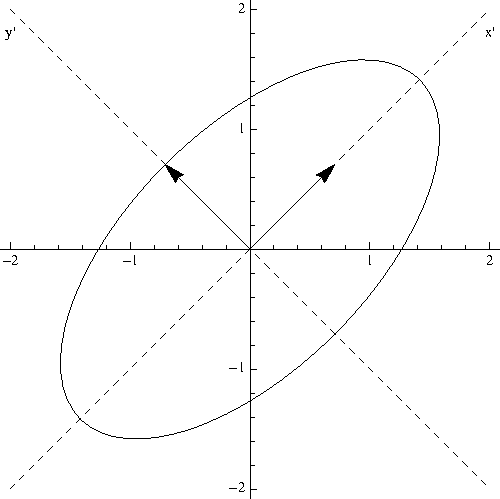
\includegraphics[width=\marginparwidth]{05-Changing-Bases/rotated-ellipse}}}%
Our goal in this example is to find the equation of an ellipse that is rotated 45 degrees, centered at the origin, and with major axis length 2 and minor axis length 1.  Looking at the picture in the margin, we can see that it would be very natural to think of this ellipse using the dotted axes rather than the normal coordinate axes.

This problem involves looking at two different coordinate systems for the plane.  
One coordinate system has the standard basis $S = \{(1,0),\,(0,1)\}$, which we will call the $xy$ coordinate system.  
The other coordinate system involves the directions along the dotted lines.  To preserve distances along the dotted lines, we'll take as our rotated basis the unit vectors in these directions: $R=\{(1/\sqrt2,1/\sqrt{2}),\, (-1/\sqrt{2},1/\sqrt{2})\}$.

In summary, we have the following coordinate systems now:
\begin{enumerate}
	\item The standard $xy$ coordinate system with basis $$S=\{(1,0),\,(0,1)\}$$ represented by the $x$ and $y$ axes.  Let $B$ be the matrix with the vectors of $S$ as columns.
	Consider the vector $\vec u = (a,b)$.  The coordinates $(x,y)_S$ of $\vec u$ relative to $S$ satisfy the matrix equation 
        $$B\bm{x\\y}_{S}=\bm{a\\b}\quad \text{or substituting in $B$,}\quad \bm{1&0\\0&1}\bm{x\\y}_{S}=\bm{a\\b}.$$
	\item The alternate $x'y'$ coordinate system with basis $$R=\{(1/\sqrt2,1/\sqrt{2}),\, (-1/\sqrt{2},1/\sqrt{2})\}$$ represented by the $x'$ ($y=x$) and $y'$ ($y=-x$) axes.  Let $C$ be the matrix with the vectors of $R$ as columns.
	Consider again the vector $\vec u = (a,b)$.  The coordinates $(x',y')_{R}$ of $(a,b)$ relative to $R$ (so $[\vec u]_{R} = (x',y')_S$) satisfy the matrix equation 
	$$C\bm{x'\\y'}_{R}=\bm{a\\b} \quad \text{or substituting in $C$,}\quad \bm{1/\sqrt2 &-1/\sqrt2\\1/\sqrt2&1/\sqrt2}\bm{x'\\y'}_{R}=\bm{a\\b}.$$
\end{enumerate}

Our goal is to find an equation of the ellipse in the $xy$ coordinate system. We know that in the $x'y'$ coordinate system an equation is $\ds \frac{(x')^2}{4}+(y')^2=1$. 
To transform an equation from using $R$ coordinates to using the normal $S$ coordinates, we need to find a matrix $P$ so that $[\vec u]_R=P[\vec u]_S$.  In other words, we need to find the change of basis matrix from $S$ to $R$ (notice the order reversed).

For every vector $\vec u =(a,b)$, we already have the equations $$B[\vec u]_{S} = [\vec u]_E=C[\vec u]_{R}\quad \quad \text{or}\quad \quad B\bm{x\\y}=C\bm{x'\\y'}.$$ 
To find $P$, we simply solve for $[\vec u]_{R}$, which gives us $C\inv B[\vec u]_{S} = [\vec u]_{R}$, or $P=C\inv B$, or more explicitly,
$$P=C\inv B = \bm{1/\sqrt2 &-1/\sqrt2\\1/\sqrt2&1/\sqrt2}\inv \bm{1&0\\0&1} = \bm{1/\sqrt2 &1/\sqrt2\\-1/\sqrt2&1/\sqrt2}.$$
We now have the transformation 
$$\bm{x'\\y'} = P\bm{x\\y} = \bm{1/\sqrt2 &1/\sqrt2\\-1/\sqrt2&1/\sqrt2}\bm{x\\y} = \bm{x/\sqrt2+y/\sqrt2\\-x/\sqrt2+y/\sqrt{2}},$$
or $x'=x/\sqrt2+y/\sqrt2, y'=-x/\sqrt2+y/\sqrt2$.

We can now answer the original question.  
The rotated ellipse had equation $\frac{(x')^2}{4}+(y')^2=1$ in the $x'y'$ coordinate system.  
We replace each $x'$ and $y'$ with $x'=x/\sqrt2+y/\sqrt2$ and $y'=-x/\sqrt2+y/\sqrt2$ to obtain the equation in terms of the normal $xy$ coordinates: $$\frac{(x/\sqrt2+y/\sqrt2)^2}4+(-x/\sqrt2+y/\sqrt2)^2=1.$$
\end{example}

Any time you encounter a problem that would be simpler in a new coordinate system, there is a change of basis matrix that can simplify the problem. 
\footnote{Different authors disagree on the use of the term ``change of basis matrix.'' 
We call $P$ the change of basis matrix \emph{from $S$ to $R$}, referring to the fact that multiplying $[\vec u]_S$ by $P$ transforms coordinates relative to $S$ into coordinates relative to $R$: $P[\vec u]_S=[\vec u]_R$.  
When working with an equation, for example, another point of view is that we can quickly convert an equation using $R$ coordinates $[\vec u]_{R}$ to an equation using $S$ coordinates $[\vec u]_S$ by replacing each instance of $[\vec u]_{R}$ with $P[\vec u]_S$.  For example, if we know that $[\vec u]_R+[\vec v]_R-2[\vec w]_R=[\vec x]_R$, then we can transform this equation to an equation involving coordinates relative to $S$ by multiplying each coordinate vector by $P$: $P[\vec u]_S+P[\vec v]_S-2P[\vec w]_S=P[\vec x]_S$.  Hence some people call $P$ the change of basis matrix \emph{from $R$ to $S$} (instead of \emph{from $S$ to $R$}).
Both phrases appear in different places and both can be considered correct. The difference lies in the context of the problem and how you plan to use the matrix. Are you focusing on what the transformation does to individual vectors, or what the transformation does to equations? 

In the equation $P[\vec u]_S = [\vec u]_{R}$, should we say $P$ is a change of basis matrix from $S$ to $R$ or from $R$ to $S$? Both can be considered correct, so make sure you know what the author means by the words ``change of basis matrix.''
}

% \begin{example}
% We'll use polar coordinates to illustrate the vocabulary difference. The transformation $x=r\cos\theta, y=r\sin\theta$, written in vector form as $ T (r,\theta)_P = (x,y)_C$, is a (nonlinear) transformation between two coordinate systems: the Cartesian and polar coordinate systems. You input vectors in polar form, and get out vectors in Cartesian form. The transformation tells us how to describe all points in the plane in either Cartesian or polar form. The transformation also tells us how to convert equations from one system to the other.  The way we use the transformation (as a transformation from polar to Cartesian, or Cartesian to polar) depends on whether we are transforming vectors or equations.    
% \begin{enumerate}
% 	\item Consider the polar vector $(r,\theta)_P = (2,\pi/6)_P$. 
% 	\marginpar{We say $T$ transforms from $S$ to $R$ when we focus on what $T$ does to individual vectors.}
% 	We obtain the Cartesian coordinates $(x,y)_C$ by applying the transformation 
% 	$$T(2,\pi/6)_P = (2\cos(\pi/6),2\sin(\pi/6))_C = (\sqrt{3},1)_C,$$ 
% 	replacing each $r$ with $2$ and each $\theta$ with $\pi/6$. 
% 	We transform a vector from polar coordinates to a vector in Cartesian coordinates. 
	
% 	\item Consider the Cartesian equation $x^2+y^2=9$ which represents a circle of radius 3 (or a collection of vectors). 
% 	\marginpar{We say $T$ transforms from $R$ to $S$ when we focus of what $T$ does to an equation (or collection of vectors).}
% 	We convert this equation to polar coordinates by replacing each $x$ with $r\cos \theta$ and each $y$ with $r\sin\theta$.
% 	The transformed equation is $(r\cos\theta)^2+(r\sin\theta)^2 = 9$, or $r^2(\cos^2\theta+\sin^2\theta)=r^2=9$, or just $r=3$. 
% 	We transform an equation from Cartesian coordinates to an equation in polar coordinates. 
% \end{enumerate}
% 	Let's emphasize the two ways of using the transformation $T[\vec u]_P=[\vec u]_C$.  
% \begin{itemize}
% 	\item $T$ transforms a vector \textit{from polar to Cartesian}. You can put in polar coordinates $(r,\theta) = [\vec u]_P$ and use $T$ to obtain Cartesian coordinates $(r\cos\theta,r\sin\theta) = [\vec u]_C$.  
% 	\item $T$ transforms equations \textit{from Cartesian to polar}. In any equation, you can replace each Cartesian coordinate of $(x,y)=[\vec u]_C$ with the corresponding polar form in $(r\cos\theta,r\sin\theta) = T[\vec u]_P$ to obtain an equation in polar coordinates. 
% \end{itemize}
% \end{example}


\section{Matrix Representations of Linear Transformations}
We showed in the last chapter that every linear transformation between two finite dimensional vector spaces has a standard matrix representation.  As a reminder, let's work a small example.
\begin{example}
The linear transformation $T\colon {\mathbb{R}}^2 \to {\mathbb{R}}^2$ defined by $T(x,y)=(2x+y,3x+4y)$ we represented in matrix form by first computing the transformation at each standard basis vector, i.e., $T(1,0)=(2,3), T(0,1)=(1,4)$, and then putting these vectors in the columns a matrix 
$A= \begin{bmatrix}2&1\\3&4\end{bmatrix}$. 
\end{example}
We compute $T(\vec x)$ by computing the matrix product $A\vec x$.  We replaced the linear transformation with matrix multiplication. We now examine how the matrix $A$ changes if we use a different basis to represent the domain and range.

Consider a linear transformation $T\colon V \to V'$ (where both $V$ and $V'$ are finite dimensional) with corresponding bases $S$ and $R$. 
How do we construct the matrix representation of $T$ relative to these bases?  
We need a matrix $A$ so that we can input coordinates relative to $S$ and get out coordinates relative to $R$.  
Notationally this matrix is written as $[T]_{S,R}$ and satisfies the equation $$[T]_{S,R}[\vec v]_S=[T(\vec v)]_{R}.$$ 
To find our matrix, we first consider everything relative to a standard basis. 
\begin{itemize}
	\item Let $A$ be the standard matrix representation of the transformation. So $$A\vec v = T(\vec v).$$
	\item Let $B$ be the matrix whose columns are the basis vectors of $S$. So $$B[\vec v]_S=[\vec v]_E=\vec v.$$
	\item Let $C$ be the matrix whose columns are the basis vectors of $R$. So $$C[\vec u]_{R}=[\vec u]_E=\vec u, \quad \text{or}\quad C[T(\vec v)]_{R}=[T(\vec v)]_E=T(\vec v).$$
\end{itemize}
On the left of $A\vec v = T(\vec v)$ we replace $\vec v$ with $B[\vec v]_S$, and on the right we replace $T(\vec v)$ with $C[T(\vec v)]_{R}$. We obtain the key equation 
$$AB[\vec v]_S=C[T(\vec v)]_{R}.$$
Multiplying both sides on the left by $C^{-1}$ gives $$[T]_{S,R}[\vec v]_S=C^{-1}AB[\vec v]_S=[T(\vec v)]_{R}.$$ This last equation requires that we input the coordinates of a vector relative to $S$, and then we get out the coordinates of the transformed vector relative to the basis $R$. This is precisely what we were looking for, which means that the matrix representation relative to $S$ and $R$ is $[T]_{S,R} = C^{-1}AB$.

\begin{example}
Consider the linear transformation $T\colon{\mathbb{R}}^2\to {\mathbb{R}}^3$ defined by $T(x,y)=(x+y,x-y,2x+3y)$. Find a matrix representation using the bases $S=\{(2,3),(-1,1)\}$ and $R=\{(1,0,0),(1,1,0),(3,2,1)\}$.  To start with, the standard matrix representation and basis matrices are 
$$
A=
\begin{bmatrix}
 1 & 1 \\
 1 & -1 \\
 2 & 3
\end{bmatrix},\,
B=
\begin{bmatrix}
 2 & -1 \\
 3 & 1
\end{bmatrix}
,\,
C=
\begin{bmatrix}
 1 & 1 & 3 \\
 0 & 1 & 2 \\
 0 & 0 & 1
\end{bmatrix}
.$$
Any vector $\vec u$ in the domain can be written as coordinates relative to $S$ using the product $ B[\vec u]_S=\vec u$.
Any vector in the image can be written as coordinates relative to $R$ using the product $C[T(\vec u)]_{R} = T(\vec u)$.  Since $A\vec u = T(\vec u)$, we replace $\vec u$ with $B[\vec u]_S$, and we replace $T(\vec u)$ with $C[T(\vec u)]_{R}$ to obtain $AB[\vec u]_S = C[T(\vec u)]_{R}$ or $C^{-1}AB[\vec u]_S=[T(\vec u)]_{R}$.  The inverse of $C$ is 
$
C^{-1}=
\begin{bmatrix}
 1 & -1 & -1 \\
 0 & 1 & -2 \\
 0 & 0 & 1
\end{bmatrix}
$.  
We can compute our matrix representation as 
$$C^{-1}AB = 
\begin{bmatrix}
 1 & -1 & -1 \\
 0 & 1 & -2 \\
 0 & 0 & 1
\end{bmatrix}
\begin{bmatrix}
 1 & 1 \\
 1 & -1 \\
 2 & 3
\end{bmatrix}
\begin{bmatrix}
 2 & -1 \\
 3 & 1
\end{bmatrix}
=
\begin{bmatrix}
 5 & 0 \\
 -1 & -2 \\
 13 & 1
\end{bmatrix}=[T]_{S,R}.
$$
\end{example}

\note{After we've drawn some pictures with different grids, we can include this paragraph: Graphically, the previous computations just give us different ways of viewing the domain and range. We can draw grids to represent the basis vectors we have chosen for the domain and range. This just gives us ways of drawing grids on the domain and range which we can then use to count out our coordinates relative to the bases chosen. }

Just as changing coordinates helps simplify problems, changing coordinates can also help us simplify transformations.  Often, we can find ``natural'' coordinates for the domain and range so that the transformation matrix $[T]_{S,R}$ is a very simple matrix.  When the matrix is very simple, it is easier to intuitively understand the transformation.

The rest of this section focuses on learning to pick a good basis for the domain and the range so that the matrix representation of $T$, $[T]_{S,R}$, is as simple as possible, in particular so that the matrix consists of the identity matrix in the upper left corner and zeroes everywhere else:
$$[T]_{S,R}=\begin{bmatrix}I&0\\0&0\end{bmatrix}.$$
To obtain this representation, we need to learn how to extend bases for the kernel and image to bases for the entire domain and range.  We'll start with this, and then apply our knowledge to matrix representations of transformations.







\subsection{The Kernel, Image, and Eigenspaces}
We have already spent time studying the three most important subspaces related to a linear transformation. These subspaces are the kernel (null space), the image (column space), and the eigenspaces. Before proceeding, let's review their definitions and why each is a subspace.
\begin{definition} Consider a linear transformation $T\colon V\to U$.
\begin{enumerate}
	\item The kernel (null space) is the set of all vectors in the domain $V$ whose image is zero: $\{\vec x \st T(\vec x)=\vec 0\}$.
	\item The image (column space) is the set of all vectors in the range $U$ whose preimage is not empty: $\{\vec y \st T(\vec x)=\vec y \text{ for some }\vec x \in V\}$.
	\item If $V=U$, for each eigenvalue $\lambda$, the eigenspace corresponding to $\lambda$ is the set of all vectors satisfying $T(\vec x) = \lambda\vec x$.  Note that eigenvalues and eigenspaces are only defined if $V=U$, or in other words, if the domain and range of $T$ are the same.
\end{enumerate}
\end{definition}
\begin{example}\label{verification of key subspaces}
Let's verify that each of these spaces is indeed a vector subspace using Theorem~\ref{thm subspace iff closed}. In what follows, we'll assume that $T$ is a linear transformation whose standard matrix representation is $A$, i.e., $T(\vec x)=A\vec x$. \note{we are being really sloppy here, since we said $V$ and $U$ are any vector space, but then we multiply vectors by matrices.  Really we should say $[T(\vec x)]_E=A[\vec x]_E$.  This sloppiness is also in the definitions above and in the discussion below.}
\begin{enumerate}
	\item Let's show that the kernel is a vector subspace of the domain. Since all the vectors in the kernel are vectors in the domain that get sent to zero, we know it is a subset of the domain.  We now show it satisfies the three requirements to be a subspace.  We will represent the zero vector of $V$ as $\vec 0_V$ and the zero vector of $U$ as $\vec 0_U$.
\begin{enumerate}
	\item Every linear transformation satisfies $T(\vec 0_V)=\vec 0_U$, so the zero vector is in the kernel because $T(\vec 0_V)$ is sent to the zero vector in $U$.  
	\item Is the sum of two vectors in the kernel still in the kernel? If $T(\vec x_1)=\vec 0_U$ and $T(\vec x_2)=\vec 0_U$ (so $\vec x_1$ and $\vec x_2$ are in the kernel), then we simply compute $T(\vec x_1+\vec x_2)=T(\vec x_1)+T(\vec x_2)=\vec 0_U+\vec 0_U=\vec 0_U$. This shows that the sum $\vec x_1+\vec x_2$ is in the kernel. 
	\item Is a scalar multiple of something in the kernel still in the kernel? If $T(\vec x)=\vec 0_U$ (so $\vec x$ is in the kernel), then we compute $T(c\vec x)=cT(\vec x)=c\vec 0_U=\vec 0_U$. This shows that the scalar multiple $c\vec x$ is in the kernel. 
\end{enumerate}

	\item Now let's show that the image is a vector subspace of the range. This proof is easiest if we utilize the fact that the span of any set of vectors is always a subspace.  Since the image of $T$ is the same as the column space of its standard matrix representation $A$, then immediately the image of $T$ is the span of the columns of $A$, hence a vector subspace.
	
	\item Now we'll show that if $V=U$, then for each eigenvalue $\lambda$ of $T$, the set of vectors that satify $T(\vec x) = \lambda \vec x$ is a vector subspace of both the domain and range.  In order to compute eigenvalues, the domain and range must be the same, so we only need to show it satisfies the three requirements to be a subspace.
\begin{enumerate}
	\item The zero vector satifies $T(\vec 0) = \vec 0 = \lambda \vec 0$, so it is in the eigenspace.  Note that $\vec 0$ is always in the eigenspace, but $\vec 0$ is not an eigenvector. The eigenvectors are the other vectors in the eigenspace.
	\item If $\vec x_1$ and $\vec x_2$ are in the eigenspace, then $T(\vec x_1)=\lambda \vec x_1$ and $T(\vec x_2)=\lambda \vec x_2$. We compute $$T(\vec x_1+\vec x_2)=T(\vec x_1)+T(\vec x_2)=\lambda \vec x_1+\lambda \vec x_2 = \lambda (\vec x_1+\vec x_2),$$ which shows that $\vec x_1+\vec x_2$ is in the eigenspace.
	\item If $\vec x$ is in the eigenspace, then $T(\vec x)=\lambda \vec x$. We then compute $T(c\vec x)=cT(\vec x)=c\lambda \vec x= \lambda (c\vec x)$. We've shown that $c\vec x$ is also in the eigenspace.
\end{enumerate}
\end{enumerate}
We have just shown that the kernel (null space), image (column space), and eigenspaces are vector spaces. You should take the time to work through the proofs above on your own. The fact that these sets of vectors are actually vector spaces means we can find a basis for each of them and talk about the coordinates of vectors in the domain or range relative to these bases.
\end{example}



\subsection{Extending a basis for a subspace to the whole space}
The three vector spaces above (kernel, image, and eigenspaces) play an important role in understanding a linear transformation. When creating a matrix representation of a linear transformation, we need a basis for the entire domain and the entire range.  The kernel provides us with a basis for part of the domain. The image provides us with a basis for part of the range.  To use these vector spaces, we must first extend a basis of a subspace to a basis for the whole space.  That is our current goal.


\subsubsection{Extending a basis for the kernel to a basis for the domain.}
The kernel of $T\colon{\mathbb{R}}^n\to{\mathbb{R}}^m$ is a vector subspace of the domain ${\mathbb{R}}^n$, so we can select a basis for the kernel. 
If the kernel has dimension $k$, we can pick $k$ vectors $\{\vec u_1, \vec u_2,\ldots, \vec u_k\}$ as the basis. 
This isn't a basis for the entire domain, so how can we pick $n-k$ other vectors $\{\vec u_{k+1},\ldots, \vec u_n\}$ so that $\{\vec u_1, \vec u_2,\ldots, \vec u_k,\vec u_{k+1},\ldots, \vec u_n\}$ is a basis for the domain ${\mathbb{R}}^n$? 
There are many ways to do this, I'll just illustrate one.  
Place your $k$ basis vectors in a matrix and augment by the $n$ by $n$ identity matrix.  This produces and $n$ by $n+k$ matrix.  Reduce this matrix, and select as your basis the $n$ pivot columns of the resulting matrix. The first $k$ vectors, the basis for the null space, will always be selected, followed by $n-k$ of the standard basis vectors.

\begin{example}
The reduced row echelon form of 
$A=
\begin{bmatrix}
 1 & 2 & 3 \\
 2 & 4 & 1
\end{bmatrix}
$
is
$
\begin{bmatrix}
 1 & 2 & 0 \\
 0 & 0 & 1
\end{bmatrix}
$.  A basis for the null space is $\{(-2,1,0)\}$. 
Putting this vector in the first column of a matrix and augmenting by the identity gives us 
$
\begin{bmatrix}
 -2 & 1 & 0 & 0 \\
 1 & 0 & 1 & 0 \\
 0 & 0 & 0 & 1\end{bmatrix}
\xrightarrow{rref}
\begin{bmatrix}
 1 & 0 & 1 & 0 \\
 0 & 1 & 2 & 0 \\
 0 & 0 & 0 & 1
\end{bmatrix}
$.
A basis for the domain is the pivot columns, namely the first, second and fourth vectors $\{(-2,1,0),(1,0,0), (0,0,1)\}$. 

\end{example}


\begin{example}
The reduced row echelon form of 
$A=
\begin{bmatrix}
 3 & 4 \\
 6 & 8
\end{bmatrix}
$
is
$
\begin{bmatrix}
 1 & \frac{4}{3} \\
 0 & 0
\end{bmatrix}
$.  A basis for the null space is $\{(-4/3,1)\}$. Putting this vector in the first column and augmenting by the identity gives us 
$$
\begin{bmatrix}
 -\frac{4}{3} & 1 & 0 \\
 1 & 0 & 1
\end{bmatrix}
\xrightarrow{rref}
\begin{bmatrix}
 1 & 0 & 1 \\
 0 & 1 & \frac{4}{3}
\end{bmatrix}
.$$
A basis for the domain is the first and second columns, namely $\{(-4/3,1),(1,0)\}$. Are there other correct answers? Of course there are, as there are infinitely many ways to choose a basis.

\end{example}

\subsubsection{Extending a basis for the kernel to a basis for the domain.}
The image of $T\colon{\mathbb{R}}^n\to{\mathbb{R}}^m$ is a vector subspace of the range ${\mathbb{R}}^m$. If the image is $r$ dimensional (recall the rank is the dimension) then we can select a basis for the image consisting of $r$ vectors $\{\vec v_1, \vec v_2,\ldots, \vec v_r\}$. How do we pick $m-r$ other vectors $\{\vec u_{k+1},\ldots, \vec u_m\}$ so that $\{\vec v_1, \vec v_2,\ldots, \vec v_r,\vec v_{r+1},\ldots, \vec v_m\}$ is a basis for the range ${\mathbb{R}}^m$? Again augment these $r$ basis vectors by the $m$ by $m$ identity matrix, and row reduce.  The $m$ pivot columns of the resulting matrix provide your basis.  This basis will always include the first $r$ vectors, and then you just add in some of the standard basis vectors.

\begin{example}
The reduced row echelon form of 
$A=
\begin{bmatrix}
 1 & 2 & 3 \\
 2 & 4 & 1
\end{bmatrix}
$
is
$
\begin{bmatrix}
 1 & 2 & 0 \\
 0 & 0 & 1
\end{bmatrix}
$.  A basis for the column space is $\{(1,2),(3,1))\}$. Since it already has 2 dimensions, there is no need to extend it to a basis for the range, we already have a basis.
\end{example}

\begin{example}
The reduced row echelon form of 
$A=
\begin{bmatrix}
 3 & 4 \\
 6 & 8
\end{bmatrix}
$
is
$
\begin{bmatrix}
 1 & \frac{4}{3} \\
 0 & 0
\end{bmatrix}
$.  A basis for the column space is $\{(3,6)\}$. Putting this vector in the first column of a matrix with 2 rows and augmenting by the identity gives us 
$
\begin{bmatrix}
 3 & 1 & 0 \\
 6 & 0 & 1
\end{bmatrix}
\xrightarrow{rref}
\begin{bmatrix}
 1 & 0 & \frac{1}{6} \\
 0 & 1 & -\frac{1}{2}
\end{bmatrix}
$.
This means that a basis for the range is the first and second columns, namely $\{(3,6),(1,0)\}$.
\end{example}

\begin{example}
The reduced row echelon form of 
$A=
\begin{bmatrix}
 1 & 2 \\
 3 & 6 \\
 -2 & -4
\end{bmatrix}
$
is
$
\begin{bmatrix}
 1 & 2 \\
 0 & 0 \\
 0 & 0
\end{bmatrix}
$.  
A basis for the column space is $\{(1,3,-2)\}$. Putting this vector in the first column of a matrix with 3 rows and augmenting by the identity gives us 
$
\begin{bmatrix}
 1 & 1 & 0 & 0 \\
 3 & 0 & 1 & 0 \\
 -2 & 0 & 0 & 1
\end{bmatrix}
\xrightarrow{rref}
\begin{bmatrix}
 1 & 0 & 0 & -\frac{1}{2} \\
 0 & 1 & 0 & \frac{1}{2} \\
 0 & 0 & 1 & \frac{3}{2}
\end{bmatrix}
$.
This means that a basis for the range is the first three columns, namely $\{(1,3,-2),(1,0,0),(0,1,0)\}$.

\end{example}

\subsubsection{Obtaining a basis for the domain and range using eigenspaces}
The last fact we will develop in this section relates to choosing a basis for both the domain and range using eigenvectors.  The first fact is that eigenvectors corresponding to different eigenvectors are always linearly independent.
\begin{theorem}
If $\vec x_1,\vec x_2,\ldots,\vec x_n$ are $n$ eigenvectors corresponding to $n$ distinct eigenvalues $\lambda_1, \lambda_2,\ldots, \lambda_n$, then the vectors $\vec x_1,\vec x_2,\ldots,\vec x_n$ are linearly independent.
\end{theorem}

\note{This is what I took out of chapter 4 about this theorem:

An important fact is that eigenvectors corresponding to different eigenvalues will always be linearly independent.  Let's first discuss why this works if we have two eigenvectors associated with two different eigenvalues.  Suppose $\vec x_1,\vec x_2$ correspond to distinct eigenvalues $\lambda_1,\lambda_2$.  Suppose in addition that $\vec x_1,\vec x_2$ are linearly dependent, which means one is a linear combination of the other $\vec x_1=c\vec x_2$.  Multiplying both sides by $A$ gives $\lambda_1 \vec x_1 = c\lambda_2\vec x_2 = \lambda_2 (c\vec x_2) = \lambda_2\vec x_1.$ This means that $\lambda_1=\lambda_2$, contrary to our assumption. Hence the two vectors must be linearly independent.  This is important enough of a fact that we will formalize it as a theorem as well.

\begin{theorem}
  If $A$ is an $n$ by $n$ matrix, and $\vec x_1,\vec x_2,...,\vec x_k$ are eigenvectors corresponding to different eigenvalues $\lambda_1, \lambda_2,...,\lambda_k$ ($\lambda_i\neq \lambda_j$ for $i\neq j$), then $\{\vec x_1,\vec x_2,...,\vec x_k\}$ is a linearly independent set.
\end{theorem}

To illustrate why this works in general, let's show it is true for three eigenvectors $\vec x_1,\vec x_2,\vec x_3$ associated with three different eigenvalues $\lambda_1,\lambda_2,\lambda_3$.  To do this, we'll build on the fact that it is true for two eigenvectors.  This method of showing a general statement is true by first showing it for a small case, then iteratively building on that small case by showing that each case implies the statement is true for the next larger case, is a very powerful technique called induction.  It is studied and used quite a bit in later math classes.

To proceed, let's consider what happens if a linear combination of the eigenvectors equals zero:
\begin{align}
  \vec 0=c_1\vec x_1+c_2\vec x_2+c_3\vec x_3.\label{eq:evec-lin-indep}
\end{align}
Now we multiply equation~\eqref{eq:evec-lin-indep} by $\lambda_3$ and by $A$ and take the difference:
\begin{align*}
  \vec 0&=\lambda_3(c_1\vec x_1+c_2\vec x_2+c_3\vec x_3)-A(c_1\vec x_1+c_2\vec x_2+c_3\vec x_3)\\
  &=\lambda_3(c_1\vec x_1+c_2\vec x_2+c_3\vec x_3)-c_1A\vec x_1-c_2A\vec x_2-c_3A\vec x_3\\
  &=c_1\lambda_3\vec x_1+c_2\lambda_3\vec x_2+c_3\lambda_3\vec x_3-c_1\lambda_1\vec x_1-c_2\lambda_2\vec x_2-c_3\lambda_3\vec x_3\\
  &= c_1(\lambda_3-\lambda_1)\vec x_1+c_2(\lambda_3-\lambda_2)\vec x_2+c_3(\lambda_3-\lambda_3)\vec x_3\\
  &=  c_1(\lambda_3-\lambda_1)\vec x_1+c_2(\lambda_3-\lambda_2)\vec x_2+\vec 0\\
  &=  c_1(\lambda_3-\lambda_1)\vec x_1+c_2(\lambda_3-\lambda_2)\vec x_2
\end{align*}

Here is the key step.  We already showed that for two eigenvectors associated with two different eigenvalues are linearly independent.  We'll use that fact to show that the next larger case is true (3 eigenvectors associated with 3 different eigenvalues).

Since $x_1$ and $x_2$ are linearly independent, we know that $c_1(\lambda_3-\lambda_1)=0$ and $c_2(\lambda_3-\lambda_2)=0$ (see Definition~\ref{def linear independence}).  Since $\lambda_3\neq \lambda_1$ and $\lambda_3\neq \lambda_2$, this means that $c_1=0$ and $c_2=0$.  Thus equation~\eqref{eq:evec-lin-indep} is actually
\begin{align*}
  \vec 0=\vec 0 + \vec 0+c_3\vec x_3,
\end{align*}
so $c_3$ must actually be zero too.  Since each of $c_1,c_2,c_3$ must be zero in Equation~\eqref{eq:evec-lin-indep}, the vectors $\vec x_1$, $\vec x_2$, and $\vec x_3$ are linearly independent by Definition~\ref{def linear independence}.

Now an analogous line of reasoning will use the truth of the statement for the case with three eigenvectors to prove the case with four eigenvectors, and so on.
}
For a proof, see problem 11.44. The key reason we want to use this theorem is that if the domain $V$ and range $V$ of a linear transformation $T\colon V\to V$ has dimension $n$, and there are $n$ distinct eigenvalues, then we can form a basis for $V$ by selecting an eigenvector corresponding to each eigenvalue. This creates a basis for $V$ by using eigenvectors. A basis chosen in this fashion will always contain a basis for the null space (as vectors in the null space are eigenvectors corresponding to the eigenvalue $\lambda = 0$). Choosing your basis vectors to be eigenvectors will greatly simplify how we view a linear transformation.


 
\begin{example}
The matrix 
$A=
\begin{bmatrix}
 1 & 4 \\
 3 & 2
\end{bmatrix}
$ has eigenvalues $5,-2$.  Corresponding eigenvectors are $(1,1)^T$ and $(-4,3)^T$ (verify this by hand or by computer). A basis for the domain and range can be chosen to be $\{(1,1),(-4,3)\}$. These vectors are linearly independent.
\end{example}
\begin{example}
The matrix 
$A=
\begin{bmatrix}
 2 & 1 & 0 \\
 1 & 2 & 0 \\
 0 & 0 & 3
\end{bmatrix}
$ has eigenvalues $3,3,1$. Notice that 3 appears with multiplicity 2.  To find the eigenvectors, we subtract 3 from the diagonal and reduce 
$
\begin{bmatrix}
 -1 & 1 & 0 \\
 1 & -1 & 0 \\
 0 & 0 & 0
\end{bmatrix}
$
to obtain
$
\begin{bmatrix}
 1 & -1 & 0 \\
 0 & 0 & 0 \\
 0 & 0 & 0
\end{bmatrix}
$
. Since there are two free variables, we can find 2 linearly independent eigenvectors corresponding to 3, namely $(1,1,0)$ and $(0,0,1)$. An eigenvector corresponding to 1 is $(-1,1,0)$. These three vectors are linearly independent, and so a basis for the domain and range is $\{ (1,1,0), (0,0,1), (-1,1,0) \}$.    
\end{example}
\begin{example}
Similar computations can be done for the matrix
$A=
\begin{bmatrix}
 2 & 1 & 1 \\
 1 & 2 & 0 \\
 0 & 0 & 3
\end{bmatrix}
$ which has eigenvalues $3,3,1$. To find the eigenvectors corresponding to 3, we subtract 3 from the diagonal and reduce 
$
\begin{bmatrix}
 -1 & 1 & 1 \\
 1 & -1 & 0 \\
 0 & 0 & 0
\end{bmatrix}
$
to obtain
$
\begin{bmatrix}
 1 & -1 & 0 \\
 0 & 0 & 1\\
 0 & 0 & 0
\end{bmatrix}
$. 
There is only one free variable, so only 1 linearly independent eigenvector corresponding to 3, namely $(1,1,0)$. There is also only one linearly independent eigenvector corresponding to 1, which is still $(-1,1,0)$. 
Some software packages return $(0,0,0)$ as a third eigenvector which the software expects you to forget, as the zero vector is by definition never an eigenvector. 
We can only obtain 2 linearly independent eigenvectors, and so a basis for the domain and range cannot be obtained just from one eigenvectors alone. For now, we augment these two vectors by the identity and row reduce to obtain 
$
\begin{bmatrix}
 1 & -1 & 1 & 0 & 0 \\
 1 & 1 & 0 & 1 & 0 \\
 0 & 0 & 0 & 0 & 1
\end{bmatrix}
\xrightarrow{rref}
\begin{bmatrix}
 1 & 0 & \frac{1}{2} & \frac{1}{2} & 0 \\
 0 & 1 & -\frac{1}{2} & \frac{1}{2} & 0 \\
 0 & 0 & 0 & 0 & 1
\end{bmatrix}
$. A basis for the domain and range which contains eigenvectors (and one other) is the first, second, and fifth columns, namely $\{ (1,1,0), (-1,1,0), (0,0,1) \}$.  The next chapter on Jordan form focuses on what to do when you cannot obtain a basis consisting of only eigenvectors. 
\end{example}













\subsection{Simplifying Matrix Representations}

%\fixthis I want to illustrate this section with graphics.  I want to show how you start with the standard basis vectors, you switch them to a different basis prior to mapping across (this just means you place different axes on the domain)  Then the transformation takes things nicely over to a different space, and the you take that space back to the standard basis.  This could be done with a sequence of 4 pictures (where you see where the unit square gets mapped).

We have already seen there are many different ways of using a matrix to represent the same transformation. 
If $B$ and $C$ are invertible matrices, and $A$ is the standard matrix representation of $T$, then $C^{-1} A B$ is a matrix representation of $T$ relative to the bases $S$ and $R$ formed from the columns of $B$ and $C$.  
Which bases $S$ and $R$ provide the best bases, or the simplest matrix representation? 
There is not really a correct answer here, as simplest is a relative term, but there are some nice bases you can choose to simplify computations.  
The kernel and image of a transformation provide us with a starting point to obtain key basis vectors needed to represent a transformation in an extremely simple way.


If you start with a basis for the kernel (null space) and extend it to a basis for the domain, then the matrix representation relative to this basis will contain columns of zeros (one for every basis vector in the null space). In other words, you can arrange your basis vectors to purposefully squash out of the matrix everything with gets mapped to zero.  Purposefully filling a matrix with lots of zeros prior to multiplication can greatly simplify computations.

\begin{example}\label{ltbasis1}
Consider the linear transformation $T\colon{\mathbb{R}}^3\to {\mathbb{R}}^2$ defined by $T(x,y,z)=(x+y-z,2x+3y+4z)$. The standard matrix representation is 
$
A=
\begin{bmatrix}
 1 & 1 & -1 \\
 2 & 3 & 4
\end{bmatrix}
$
whose rref is
$
\begin{bmatrix}
 1 & 0 & -7 \\
 0 & 1 & 6
\end{bmatrix}
$. A basis for the kernel (null space) is $(7,-6,1)$. We extend this to a basis for the domain by augmenting by the identity and reducing, 
$
\begin{bmatrix}
 7 & 1 & 0 & 0 \\
 -6 & 0 & 1 & 0 \\
 1 & 0 & 0 & 1
\end{bmatrix}
\xrightarrow{rref}
\begin{bmatrix}
 1 & 0 & 0 & 1 \\
 0 & 1 & 0 & -7 \\
 0 & 0 & 1 & 6
\end{bmatrix}
$, which means that $S=\{(7,-6,1),(1,0,0),(0,1,0)\}$ is a basis for the domain. Using $E=\{(1,0),(0,1)\}$ as a basis for the range, we compute the matrix representation of $T$ relative to the bases $S$ and $E$ by noting 
$$C=
\begin{bmatrix}
1 & 0\\
0 & 1
\end{bmatrix}=C^{-1},
A=
\begin{bmatrix}
 1 & 1 & -1 \\
 2 & 3 & 4
\end{bmatrix}, 
B=
\begin{bmatrix}
 7 & 1 & 0 \\
 -6 & 0 & 1 \\
 1 & 0 & 0
\end{bmatrix},
C^{-1}AB= 
\begin{bmatrix}
 0 & 1 & 1 \\
 0 & 2 & 3
\end{bmatrix} = [T]_{S,E}.$$ 
Notice how this made the entire first column of the matrix zero. If we rearrange the basis vectors of $S$ so that the vectors in the null space are at the end, $S=\{(1,0,0),(0,1,0),(7,-6,1)\}$, then our matrix is simply $[T]_{S,E} = \begin{bmatrix}
 1 & 1 &0\\
 2 & 3 &0
\end{bmatrix}$. We just moved the column of zeros to the end of the matrix instead of the beginning. Putting the column of zeros at the end is done in practice to make it easy to remember that we can ignore the last column (or columns) of the matrix (instead of the first).

\end{example}

After picking a basis for the domain which contains the kernel, let's carefully construct a basis for the range to make our matrix representation extremely nice.  
If $k$ is the dimension of the kernel and $S=\{\vec v_1,\vec v_2,\ldots,\vec v_n\}$ is a basis for the domain (whose last $k$ vectors are in the kernel - they were moved to the end), then consider the $n-k$ vectors $\{T(\vec v_{1}),\ldots,T(\vec v_{n-k})\}$ which are nonzero vectors in the image.  Since the image has to have dimension $n-k$, these $n-k$ vectors form a basis for the image. We can extend them to a basis $R$ for the range (augmenting by the identity and reducing). The matrix representation of $T$ relative to the bases $S$ and $R$ will always be a matrix which consists of all zeros and $n-k$ 1's (what can be simpler than zeros and 1's).  This representation of $T$ illustrates how the kernel and image can be use to obtain an extremely nice form for our matrix representation.  Mathematicians who work with maps in high dimensions often start by placing things in ``general position'' which is very similar to picking nice bases so that their maps consist of identity and zero transformations, precisely what we are doing now.  Let's look at examples.



\begin{example}
Consider the linear transformation from example \ref{ltbasis1} $T\colon{\mathbb{R}}^3\to {\mathbb{R}}^2$ defined by $T(x,y,z)=(x+y-z,2x+3y+4z)$. Using the bases $S=\{(1,0,0),(0,1,0),(7,-6,1)\}$ and $E=\{(1,0),(0,1)\}$ (the standard basis for the plane), the matrix representation of $T$ relative to these bases is  
$[T]_{S,E} = \begin{bmatrix}
 1 & 1 &0\\
 2 & 3 &0
\end{bmatrix}$. 
Let's pick a different basis for the range.  A basis for the image is $R = \{(1,2),(1,3)\}$, the nonzero columns of $[T]_{S,E}$. 
The matrix representation of $T$ relative to the bases $S$ and $R$ is then found using 
$$C=
\begin{bmatrix}
1 & 1\\
2 & 3
\end{bmatrix},
C^{-1} = 
\frac{1}{1}
\begin{bmatrix}
3 & -1\\
-2 & 1
\end{bmatrix},
A=
\begin{bmatrix}
 1 & 1 & -1 \\
 2 & 3 & 4
\end{bmatrix}, 
B=
\begin{bmatrix}
 1 & 0 &7\\
 0 & 1 &-6\\
 0 & 0 &1
\end{bmatrix},
$$
$$
\quad \text {and so} \quad 
[T]_{S,R} =C^{-1}AB= 
\begin{bmatrix}
 1 & 0 & 0 \\
 0 & 1 & 0
\end{bmatrix} .$$ 
Not only have we made the last column zero, but we have also placed the identity matrix in the upper left corner of the matrix. This will happen in general, even with bigger matrices.
\end{example}

\begin{example}
Let's look at a much larger example. 
Perform the computations on the computer to verify the work below. 
Consider the transformation $T(x,y,z,w)=(2x-y,y+z,2x+z,x+w)$.  
The standard matrix representation of $T$ is 
$$
A=
\begin{bmatrix}
 2 & -1 & 0 & 0 \\
 0 & 1 & 1 & 0 \\
 2 & 0 & 1 & 0 \\
 1 & 0 & 0 & 1
\end{bmatrix}
\xrightarrow{rref}
\begin{bmatrix}
 1 & 0 & 0 & 1 \\
 0 & 1 & 0 & 2 \\
 0 & 0 & 1 & -2 \\
 0 & 0 & 0 & 0
\end{bmatrix}
.$$ 
A basis for the kernel is $(-1,-2,2,1)$. 
We extend this to a basis for the domain by augmenting by the identity and reducing, 
$$
\begin{bmatrix}
 -1 & 1 & 0 & 0 & 0 \\
 -2 & 0 & 1 & 0 & 0 \\
 2 & 0 & 0 & 1 & 0 \\
 1 & 0 & 0 & 0 & 1
\end{bmatrix}
\xrightarrow{rref}
\begin{bmatrix}
 1 & 0 & 0 & 0 & 1 \\
 0 & 1 & 0 & 0 & 1 \\
 0 & 0 & 1 & 0 & 2 \\
 0 & 0 & 0 & 1 & -2
\end{bmatrix},
$$. 
A basis for the domain is $S=\{(1,0,0,0),(0,1,0,0),(0,0,1,0),(-1,-2,2,1)\}$, where we placed the vector in the kernel at the end. 
Using the standard basis for the range, we compute the matrix representation of $T$ relative to the bases $S$ and $E$ by noting 
$$C=I=C^{-1},
A=
\begin{bmatrix}
 2 & -1 & 0 & 0 \\
 0 & 1 & 1 & 0 \\
 2 & 0 & 1 & 0 \\
 1 & 0 & 0 & 1
\end{bmatrix}, 
B=
\begin{bmatrix}
 1 & 0 & 0 & -1 \\
 0 & 1 & 0 & -2 \\
 0 & 0 & 1 & 2 \\
 0 & 0 & 0 & 1
\end{bmatrix},$$
$$\text{and so}\quad [T]_{S,E} = C^{-1}AB= 
\begin{bmatrix}
 2 & -1 & 0 & 0 \\
 0 & 1 & 1 & 0 \\
 2 & 0 & 1 & 0 \\
 1 & 0 & 0 & 0
\end{bmatrix}.$$ 
The last column now contains only zeros. Now that we've got a basis for the domain that contain a basis for the kernel, we pick a different basis for the range.
The vectors $\{(1,0,0,0),(0,1,0,0),(0,0,1,0)$ have images $\{(2,0,2,1),(-1,1,0,0),(0,1,1,0)\}$ (the nonzero columns of the previous matrix). These nonzero columns provide a basis for the image.  Extend this set to a basis for the range by augmenting by the identity and reducing
$$\begin{bmatrix}
 2 & -1 & 0 & 1 & 0 & 0 & 0 \\
 0 & 1 & 1 & 0 & 1 & 0 & 0 \\
 2 & 0 & 1 & 0 & 0 & 1 & 0 \\
 1 & 0 & 0 & 0 & 0 & 0 & 1
\end{bmatrix}
\xrightarrow{rref}
\begin{bmatrix}
 1 & 0 & 0 & 0 & 0 & 0 & 1 \\
 0 & 1 & 0 & 0 & 1 & -1 & 2 \\
 0 & 0 & 1 & 0 & 0 & 1 & -2 \\
 0 & 0 & 0 & 1 & 1 & -1 & 0
\end{bmatrix}.
$$ 
We select the pivot columns $R = \{(2,0,2,1),(-1,1,0,0),(0,1,1,0),(1,0,0,0)\}$ as a basis for the range. 
The matrix representation of $T$ relative to the bases $S$ and $R$ is then found using 
$$C=
\begin{bmatrix}
 2 & -1 & 0 & 1 \\
 0 & 1 & 1 & 0 \\
 2 & 0 & 1 & 0 \\
 1 & 0 & 0 & 0
\end{bmatrix},
C^{-1} = \frac{1}{1}
\begin{bmatrix}
 0 & 0 & 0 & 1 \\
 0 & 1 & -1 & 2 \\
 0 & 0 & 1 & -2 \\
 1 & 1 & -1 & 0
\end{bmatrix},
B=
\begin{bmatrix}
 1 & 0 & 0 & -1 \\
 0 & 1 & 0 & -2 \\
 0 & 0 & 1 & 2 \\
 0 & 0 & 0 & 1
\end{bmatrix},$$
$$[T]_{S,R} = C^{-1}AB= 
\begin{bmatrix}
 1 & 0 & 0 & 0 \\
 0 & 1 & 0 & 0 \\
 0 & 0 & 1 & 0 \\
 0 & 0 & 0 & 0
\end{bmatrix}.$$ In the first step we made the last column zero. In this step we put the identity matrix in the upper left corner of the matrix, with a row of zeros at the bottom. 
This is perhaps the simplest form you can obtain.
\end{example}

Every linear transformation $T\colon V\to V'$ of rank $r$ can be represented by a matrix of the form $[T]_{S,R}=\bm{I&0\\0&0}$, where the only nonzero entries are $r$ 1's, located in the upper left corner. To obtain this basis require the following steps: 
\begin{enumerate}
	\item Find a basis for the kernel.
	\item Extend the basis for the kernel to a basis $S$ for the domain, placing the vectors in the kernel at the end.
	\item Find the images each basis vector for the domain. The nonzero vectors form a basis for the image.
	\item Extend the basis for the image to a basis $R$ for the range, placing the vectors in the image at the front.  
\end{enumerate}
Along the way, there are infinitely many choices you can make at each step.  The interesting thing is that regardless of the choices we make, we will always obtain the exact same form $[T]_{S,R}=\bm{I&0\\0&0}$. In the next section we will focus on what happens if $T\colon V\to V$ has the same domain and range, and we use the same basis $S$ for both the domain and range. 


%As a side note, I would like to include Fourier Coefficients here (just as a brief 3 minute illustration in class).


\section{Similar Matrices}
If a linear transformation $T\colon V\to V$ has the same domain as range, then we often want to pick the same basis $S$ for both the domain and range. 
The coordinates of $\vec u$ relative to $S$ are written $P[\vec u]_S = [\vec u]_E$, where $P$ is the matrix whose columns are the basis vectors in $S$. 
If $A$ is the standard matrix representation of the linear transformation, then we write 
$$A[\vec u]_E = [T(\vec u)]_E.$$  
Replacing $[\vec u]_E$ on the left with $P[\vec u]_S = [\vec u]_E$, and replacing $[T(\vec u)]_E$ on the right with $P[T(\vec u)]_S = [T(\vec u)]_E$ gives the matrix equation 
$$AP[\vec u]_S = P[T(\vec u)]_S\quad \text{or}\quad P^{-1}AP [\vec u]_S = [T(\vec u)]_S.$$ The matrix representation of $T$ relative to the basis $S$ is $[T]_{S,S}=[T]_S = P^{-1}AP$ (we only write one $S$). 
This new matrix is found by multiplying on the right by $P$, and on the left by $P\inv$.    

\begin{definition}
We say $A$ and $B$ are similar matrices, and write $A\sim B$ if there exists an invertible matrix $P$ such that $B=P^{-1}AP$.
\end{definition}

Similar matrices have many properties that we'll put into a theorem. 

\begin{theorem}
\begin{enumerate}
	\item Every matrix is similar to itself, $A\sim A$. (We say similarity is reflexive.)
	\item If $A\sim B$, then $B\sim A$. (We say similarity is symmetric.)
	\item If $A\sim B$ and $B\sim C$, then $A\sim C$. (We say similarity is transitive.)
	\item Similar matrices have the same determinant, eigenvalues, rank, and nullity.
\end{enumerate}
\end{theorem}
\begin{proof} Let's take a moment to justify why each of the facts above is true.  Any relationship between sets which satisfies the first three facts above is said to be an equivalence relation.  You will study equivalence relations in more depth in future classes.
\begin{enumerate}
	\item Every matrix $A$ is similar to itself, because letting $P=I$, the identity matrix, gives $A=I^{-1}AI$. 
	\item If $A$ is similar to $B$, then there is some $P$ such that $B=P^{-1}AP$, then multiplying both sides on the right by $P^{-1}$ and on the left by $P$ gives $PBP^{-1}=A$, or $A = (P^{-1})^{-1}BP^{-1}$ (as $(P^{-1})^{-1}=P$). Hence $B$ is similar to $A$.  
	\item If $A$ is similar to $B$ and $B$ is similar to $C$, then $B=P^{-1}AP$ and $C=Q^{-1}BQ$.  We replace $B$ in the second equation to obtain $C=Q^{-1}BQ = Q^{-1}P^{-1}APQ = R^{-1}AR$ where $R=PQ$ and recall that $R^{-1} = Q^{-1}P^{-1}$ (inverting a product requires inverting each factor and reversing the order of multiplication). This shows that $A$ is similar to $C$.
	\item If $A$ and $B$ are similar, then $B=P\inv A P$. Taking determinants gives $|B|=|P^{-1}AP| = |P^{-1}||A||P| = |P|^{-1}|A||P| =|A|$, hence similar matrices have the same determinant. 
	
	To show they have the same eigenvalues, we compute 
	\begin{align*}
	|B-\lambda I|&=|P^{-1}AP-\lambda I|\\
	&=|P^{-1}AP-\lambda P^{-1}IP|\\
	&=|P^{-1}(A-\lambda I)P|\\
	&=|P^{-1}||(A-\lambda I)||P|,
	\end{align*} 
	which means $|B-\lambda I| = 0 $ if and only if $|P^{-1}||(A-\lambda I)||P|=0$. The latter equals zero if and only if $|(A-\lambda I)|=0$. Hence $B$ and $A$ have the same eigenvalues.
	
  We now show the rank and nullity are the same. We'll show that for every vector in the null space of $A$, there is a corresponding vector in the null space of $B$ (so the nullity of $A$ cannot be larger than the nullity of $B$).  Then by similarity, we interchange the roles of $A$ and $B$ (so the nullity of $B$ cannot be larger than the nullity of $A$). If $\vec x$ is in the null space of $A$, then $A\vec x = \vec 0$. The vector $\vec y = P\inv \vec x$ is in the null space of $B$ since $B\vec y = P\inv A P (P\inv \vec x) = P A \vec x = P\vec 0 = \vec 0.$ Because $P$ is invertible, every vector in the null space of $A$ corresponds to a different vector in the null space of $B$, which means that the nullity of $A$ cannot be larger than the nullity of $A$.  By similarity, the nullity of $B$ cannot be larger than the nullity of $A$, so the nullity of both is the same.  Since rank plus nullity equals the number of columns for both matrices, we know that the ranks are the same as well.     
\end{enumerate}
\end{proof}

Similar matrices are just different ways of viewing the same linear transformation in terms of a different basis. The facts above show that the determinant, eigenvalues, rank, and nullity of a linear transformation do not depend on the basis chosen. They are important numbers which belong to any linear transformation (regardless of the basis) and can be discussed without referencing the basis vectors (or obtaining a matrix).


\begin{example}
 Consider the matrix
 $A=  
\begin{bmatrix}
 1 & 4 \\
 2 & 3
\end{bmatrix} 
$. Let
$P=
\begin{bmatrix}
 2 & 9 \\
 1 & 4
\end{bmatrix} 
$ which means 
$P^{-1} = 
\begin{bmatrix}
 -4 & 9 \\
 1 & -2
\end{bmatrix} 
$. The matrix representation of $T$ relative to $S$ (the column vectors of $P$) is the similar matrix 
$$
P^{-1}AP=\begin{bmatrix}
 -4 & 9 \\
 1 & -2
\end{bmatrix} 
 \begin{bmatrix}
 1 & 4 \\
 2 & 3
\end{bmatrix} 
\begin{bmatrix}
 2 & 9 \\
 1 & 4
\end{bmatrix} 
=
\begin{bmatrix}
 39 & 170 \\
 -8 & -35
\end{bmatrix} 
.$$

\item

Now consider the same matrix
 $A$, but pick a different matrix 
$P=
\begin{bmatrix}
 1 & -2 \\
 1 & 1
\end{bmatrix} 
$ which means 
$P^{-1} = 
\begin{bmatrix}
 \frac{1}{3} & \frac{2}{3} \\
 -\frac{1}{3} & \frac{1}{3}
\end{bmatrix} 
$. The matrix representation of $T$ relative to $S$ (the column vectors of $P$) is the similar matrix 
$$
P^{-1}AP=\begin{bmatrix}
 \frac{1}{3} & \frac{2}{3} \\
 -\frac{1}{3} & \frac{1}{3}
\end{bmatrix} 
 \begin{bmatrix}
 1 & 4 \\
 2 & 3
\end{bmatrix} 
\begin{bmatrix}
 1 & -2 \\
 1 & 1
\end{bmatrix} 
=
\begin{bmatrix}
 5 & 0 \\
 0 & -1
\end{bmatrix} 
.$$  Notice how this choice of basis resulted in a diagonal matrix. The next section shows how you can find the right matrix $P$ so that $A$ is similar to a diagonal matrix.
\end{example}


\subsection{Diagonalizing a Matrix - Picking the ``Best Basis'' }
Recall the following: we say that $A$ is similar to $B$ if $B=P^{-1}AP$ for some invertible matrix $A$. 
This is equivalent to writing $AP=PB$, for some invertible matrix $P$. 
In this section, we will show that choosing $P$ to be a matrix of eigenvectors, when possible, yields a diagonal matrix $D$ that is similar to  $A$, so that $AP=PD$. This process is called diagonalization.  We'll connect diagonalization to a geometric visualization of linear transformations. We'll also show how diagonalization yields a vector field with specified properties. The next chapter explore this topic more and shows how diagonalization greatly simplifies computing powers of matrices and its connection to differential equations.

Let $A$ be an $n$ by $n$ matrix.  Suppose $A$ has $n$ linearly independent eigenvectors $\{\vec x_1,\vec x_2, \ldots, \vec x_n\}$. Let $P = [\vec x_1~\vec x_2~\cdots~\vec x_n]$ be the matrix whose columns are these independent eigenvectors of $A$.  We compute the matrix product
\begin{align*}
AP &= A[\vec x_1~\vec x_2~\vec x_3~\cdots~\vec x_n] \\
&= [A\vec x_1~A\vec x_2~A\vec x_3~\cdots~A\vec x_n] \\
&= [\lambda_1\vec x_1~\lambda_2\vec x_2~\lambda_3\vec x_3~\cdots~\lambda_n\vec x_n] \\
&= [\vec x_1~\vec x_2~\vec x_3~\cdots~\vec x_n]
\bm{
\lambda_1&0&0&\cdots&0\\
0&\lambda_2&0&\cdots&0\\
0&0&\lambda_3&\ddots&0\\
\vdots&\vdots&\ddots&\ddots&\vdots\\
0&0&0&\cdots&\lambda_n\\}\\
&= PD\end{align*} where $D$ is the diagonal matrix of eigenvalues (written in the same order as the order in which the eigenvectors are written in $P$).  
So when $P$ is a matrix of independent eigenvectors, we have $$AP = PD\quad \text{or}  P^{-1}AP=D.$$ The matrix $A$ is similar to the diagonal matrix $D$, using $P$ as the similarity matrix. 
This process is called diagonalizing a matrix. 
Notice that if $A$ is similar to $D$, then $AP=PD$ must hold, which means that $P$ must be a matrix whose columns are linearly independent eigenvectors (so that $P$ has an inverse). We have the following key theorem.
\begin{theorem}
A matrix is diagonalizable if and only if there are $n$ linearly independent eigenvectors. For any similarity matrix $P$ that diagonalizes $A$ (i.e., $D = P\inv A P$), the columns of $P$ must be $n$ linearly independent eigenvectors. The $k$th eigenvector corresponds to an eigenvalue of $A$ which is the $k$th entry on the diagonal of $D$. 
\end{theorem}

\begin{example}
Consider the linear transformation $T(x,y) = (x+4y,2x+3y)$ whose standard matrix representation is
$A=  
\begin{bmatrix}
 1 & 4 \\
 2 & 3
\end{bmatrix} 
$. The eigenvalues are 5 and -1 (verify this by hand on 2 by 2 matrices, but use the computer to do anything bigger). Corresponding eigenvectors are $(1,1)$ and $(-2,1)$, so let $S=\{(1,1),(-2,1)\}$ be a basis for the plane.  Form the matrix 
$P=
\begin{bmatrix}
 1 & -2 \\
 1 & 1
\end{bmatrix} 
$ whose columns are the eigenvectors. The inverse of $P$ is 
$P^{-1} = 
\begin{bmatrix}
 \frac{1}{3} & \frac{2}{3} \\
 -\frac{1}{3} & \frac{1}{3}
\end{bmatrix} 
$. The matrix representation of $T$ relative to $S$ is 
$$
P^{-1}AP=\begin{bmatrix}
 \frac{1}{3} & \frac{2}{3} \\
 -\frac{1}{3} & \frac{1}{3}
\end{bmatrix} 
 \begin{bmatrix}
 1 & 4 \\
 2 & 3
\end{bmatrix} 
\begin{bmatrix}
 1 & -2 \\
 1 & 1
\end{bmatrix} 
=
\begin{bmatrix}
 5 & 0 \\
 0 & -1
\end{bmatrix} 
,$$ a diagonal matrix.  We have diagonalized $A$ (or found a diagonal representation of the linear transformation $T$). Type this example into the Maple introduction to visual what we have just done.
 
\end{example}

\begin{example} \label{multiplicityex1}
Let's now repeat with a 3 by 3 matrix. 
Consider the linear transformation defined by the matrix
$A=  
\begin{bmatrix}
 2 & 1 & 0 \\
 1 & 2 & 0 \\
 0 & 0 & 3
\end{bmatrix} 
$. The eigenvalues are 3,3,1 (use the computer). Corresponding eigenvectors are $(0,0,1), (1,1,0),$ and $(-1,1,0)$, so let $S=\{(0,0,1), (1,1,0),(-1,1,0)\}$ be a basis for our domain and range.  Form the matrix 
$P=
\begin{bmatrix}
 0 & 1 & -1 \\
 0 & 1 & 1 \\
 1 & 0 & 0
\end{bmatrix} 
$ whose columns are the eigenvectors. The inverse of $P$ is 
$P^{-1} = 
\begin{bmatrix}
 0 & 0 & 1 \\
 \frac{1}{2} & \frac{1}{2} & 0 \\
 -\frac{1}{2} & \frac{1}{2} & 0
\end{bmatrix} 
$. The matrix representation of $T$ relative to $S$ is 
$$
P^{-1}AP=
\begin{bmatrix}
 0 & 0 & 1 \\
 \frac{1}{2} & \frac{1}{2} & 0 \\
 -\frac{1}{2} & \frac{1}{2} & 0
\end{bmatrix} 
 \begin{bmatrix}
 2 & 1 & 0 \\
 1 & 2 & 0 \\
 0 & 0 & 3
\end{bmatrix} 
\begin{bmatrix}
 0 & 1 & -1 \\
 0 & 1 & 1 \\
 1 & 0 & 0
\end{bmatrix} 
=
\begin{bmatrix}
 3 & 0 & 0 \\
 0 & 3 & 0 \\
 0 & 0 & 1
\end{bmatrix} 
,$$ a diagonal matrix.  We have diagonalized $A$ (or found a diagonal representation of the linear transformation $T$). Type this example into the Maple introduction to visual what we have just done.
\end{example}
This last example shows that not every matrix can be diagonalized.  Remember that in order to diagonalize a matrix, you must be able to find $n$ linearly independent eigenvectors. After this example, we'll state the general results.

\begin{example} \label{multiplicityex2}
Consider the linear transformation defined by the matrix
$A=  
\begin{bmatrix}
 2 & 1 & 1 \\
 1 & 2 & 0 \\
 0 & 0 & 3
\end{bmatrix} 
$. 
The eigenvalues are 3,3,1 (use a computer). Corresponding bases for the eigenspaces are $(0,0,1)$ for 3 and $(-1,1,0)$ for 1. There are only 2 linearly independent eigenvectors.  In this case, there are not enough linearly independent eigenvectors to diagonalize this matrix.  Jordan Form is a method of handling these kinds of matrices, which we will study in the next chapter. 
\end{example}


\subsection{Algebraic and Geometric Multiplicity}
Is every $n$ by $n$ matrix diagonalizable?  
Does every $n$ by $n$ matrix have $n$ linearly independent eigenvectors? 
The previos example shows that the answer is no. 
There are matrices which cannot be diagonalized. 
So what does it take for a matrix to not be diagonalizable. 
To not have enough eigenvectors, 
an eigenvalue must appear with multiplicity greater than 1, but not have the same number of corresponding linearly independent eigenvectors. We now make some definitions to simplify talking about this issue.
\begin{definition}
The \textbf{algebraic multiplicity} of an eigenvalue is the number of times that eigenvalues appears as a root of the characteristic polynomial.

The \textbf{geometric multiplicity} of an eigenvalue is the dimension of the corresponding eigenspace. 

If the geometric multiplicity of an eigenvalue is less than the algebraic multiplicity, then we say the eigenvalue is \textbf{deficient} (there were not enough eigenvectors in the eigenspace).
\end{definition}


\begin{theorem}
The geometric multiplicity is always less than or equal to the algebraic multiplicity.  A matrix is diagonalizable if and only if the algebraic multiplicity of each eigenvalue equals the geometric multiplicity of each eigenvalue. 
If all the eigenvalues are distinct, then $A$ is diagonalizable.
\end{theorem}

\begin{example}
Let's revisit examples \ref{multiplicityex1} and  \ref{multiplicityex2} to compute the algebraic and geometric multiplicity of each eigenvalue.  For both matrices, the characteristic polynomial has zeros $3,3,1$, which means that the algebraic multiplicity of $\lambda=3$ is 2, and the algebraic multiplicity of $\lambda=1$ is 1. 

For example \ref{multiplicityex1},
a basis for the $E_3$ (the eigenspace corresponding to $\lambda = 3$) is $\{(0,0,1), (1,1,0)\}$, and a basis for $E_1$ is $\{(-1,1,0)\}$. The geometric multiplicity of $\lambda =3$ is 2, and the geometric multiplicity of $\lambda = 1$ is $1$.  Because the geometric and algebraic multiplicities match, this matrix is diagonalizable.

For example \ref{multiplicityex2}, a basis for $E_3$ is $\{(0,0,1)\}$. The geometric multiplicity of $\lambda = 3$ is only 1, whereas the algebraic multiplicity is 2. The eigenvalue $\lambda=3$ is deficient; it's missing an eigenvector.  For this reason, the matrix is not diagonalizable.
\end{example}

\subsection{Physical Applications of Diagonalization}
Suppose we have a vector field that pushes objects straight outwards in the direction $(1,1)$ with a force that is triple the distance from the origin, and pulls objects towards the origin in the direction $(-1,1)$ with a force that is equal to the distance to the origin. In other words, our vector field has eigenvectors $(1,1)$ and $(-1,1)$ with corresponding eigenvalues $3$ and $-1$. Is this enough information to determine the entire vector field?  We seek a matrix $A$ with eigenvectors $(1,1)$ and $(-1,1)$ with eigenvalues 3 and $-1$.  The principle of diagonalization comes to our aide.  Because $A$ has two linearly independent eigenvectors, we know that it is diagonalizable where $$ P = \bm{1&-1\\1&1}, D = \bm{3&0\\0&-1},P\inv =\frac12\bm{1&1\\-1&1}. $$ We solve the equation $D = P\inv A P$ for $A$ to obtain 
$$A = PDP\inv = \bm{1&-1\\1&1}\bm{3&0\\0&-1}\frac12\bm{1&1\\-1&1} = \bm{1&2\\2&1}.$$
We just obtained the matrix which represents our vector field. All we needed to know was the eigenvalues and eigenvectors, something than can be seen and measured physically in a vector field. So we now have the ability to take a physical moving force and use diagonalization to connect it back to matrices.  

As time permits, I will add one other application related to computer graphics. Stay tuned.



%%% Local Variables: 
%%% mode: latex
%%% TeX-master: "../linear-algebra"
%%% End: 

